% !TEX root = ../om_ts_06.tex

\begin{frame} % название фрагмента

\videotitle{Буковка I}

\end{frame}



\begin{frame}{Буковка I: план}
  \begin{itemize}[<+->]
    \item Стационарность $ARMA$. 
    \item Определение $ARIMA$.
    \item Нужно ли переходить к разностям?
  \end{itemize}

\end{frame}


\begin{frame}
  \frametitle{$ARMA$ процесс}

  \begin{block}{Определение}
    $ARMA(p, q)$ процессом с несократимым уравнением 
    \[
      y_t = c + \beta_1 y_{t-1} + \ldots + \beta_p y_{t-p} + u_t + \alpha_1 u_{t-1} + \ldots + \alpha_q u_{t-q}, 
    \]
    где $(u_t)$ — белый шум, $\beta_p \neq 0$ и $\alpha_q \neq 0$, называется 
    решение этого уравнения вида $MA(\infty)$ относительно $(u_t)$.
  \end{block}

  \pause  
  \begin{block}{Определение с лагами}
    $ARMA(p,q)$ процессом с уравнением 
    \[
      P(L)y_t = c + Q(L)u_t, 
    \]
    где $(u_t)$ — белый шум, $P(L)$ степени $p$ и $Q(L)$ степени $q$ несократимы, $P(0)=Q(0)=1$, 
    называется решение этого уравнения вида $MA(\infty)$ относительно $(u_t)$.  
  \end{block}
\end{frame}

\begin{frame}
  \frametitle{Нюансы}

  \begin{itemize}
    \onslide<1->{\item Процесс $y_t \sim ARMA(p, q)$ стационарен \alert{по определению}:}
    
    \onslide<2->{$\E(y_t) = \mu_y$, $\Var(y_t) = \gamma_0$, $\Cov(y_t, y_{t-k}) = \gamma_k$.}

    \onslide<3->{\item В \alert{канонической записи} $ARMA(p, q)$ процесса $P(L) y_t = c+ Q(L) u_t$ у полинома $P(L)$
    все корни $\abs{\ell} > 1$.}

    \onslide<4->{Возможны неканонические варианты. }

    \onslide<5->{\item При оценке $ARMA(p, q)$ процесса методом максимального правдоподобия эти ограничения наложены \alert{а-приори}. }
    
    \onslide<6->{Есть упрощённые варианты правдоподобия.}
  \end{itemize}

\end{frame}


\begin{frame}
  \frametitle{Что делать с нестационарными процессами?}

  \begin{block}{Определение}
    Случайный процесс $(y_t)$ называется $ARIMA(p, 1, q)$ процессом относительно белого шума $(u_t)$, 
    если $(y_t)$ нестационарен, но $\Delta y_t$ — стационарный $ARMA(p, q)$ процесс относительно белого шума $(u_t)$.  
  \end{block}

  \pause

  \begin{block}{Определение}
    Случайный процесс $(y_t)$ называется $ARIMA(p, 2, q)$ процессом относительно белого шума $(u_t)$, 
    если $(y_t)$ и $(\Delta y_t)$ нестационарны, но $\Delta^2 y_t$ — стационарный $ARMA(p, q)$ процесс относительно белого шума $(u_t)$.  
  \end{block}

  \pause
  $\Delta y_t = y_t - y_{t-1}$ и $\Delta^2 y_t = \Delta y_t - \Delta y_{t-1}$

  \pause 
  ARIMA — \alert{A}uto\alert{R}egressive \alert{I}ntegrated \alert{M}oving \alert{A}verage
  
\end{frame}

\begin{frame}
  \frametitle{Как выбрать?}
  
  $ARIMA(p, 0, q)$ или $ARIMA(p, 1, q)$ или $ARIMA(p, 2, q)$
  \begin{itemize}
    \onslide<2->{\item Посмотреть на \alert{график}!}
    
    \onslide<3->{График стационарного процесса колеблется в \alert{полосе постоянной ширины} вокруг своего ожидания.}

    \onslide<4->{\item Оценить все эти модели и выбрать наилучшую по \alert{кросс-валидации}.}
    
    \onslide<5->{Затратно по времени!}

    \onslide<6->{\item \alert{Применять $AIC$ нельзя}!}
    
    \onslide<7->{$\ln L(y_1, \ldots, y_n \mid \theta)$ и $\ln L(y_2, \ldots, y_n \mid \theta, y_1)$ и $\ln L(y_3, \ldots, y_n \mid \theta, y_1, y_2)$
    несравнимы!}
    \onslide<8->{\item Есть \alert{тесты на единичный корень}!}
    
    \onslide<9->{ADF, KPSS, PP, \ldots}
  \end{itemize}

\end{frame}

\begin{frame}
  \frametitle{Выбираем «на глазок»}
  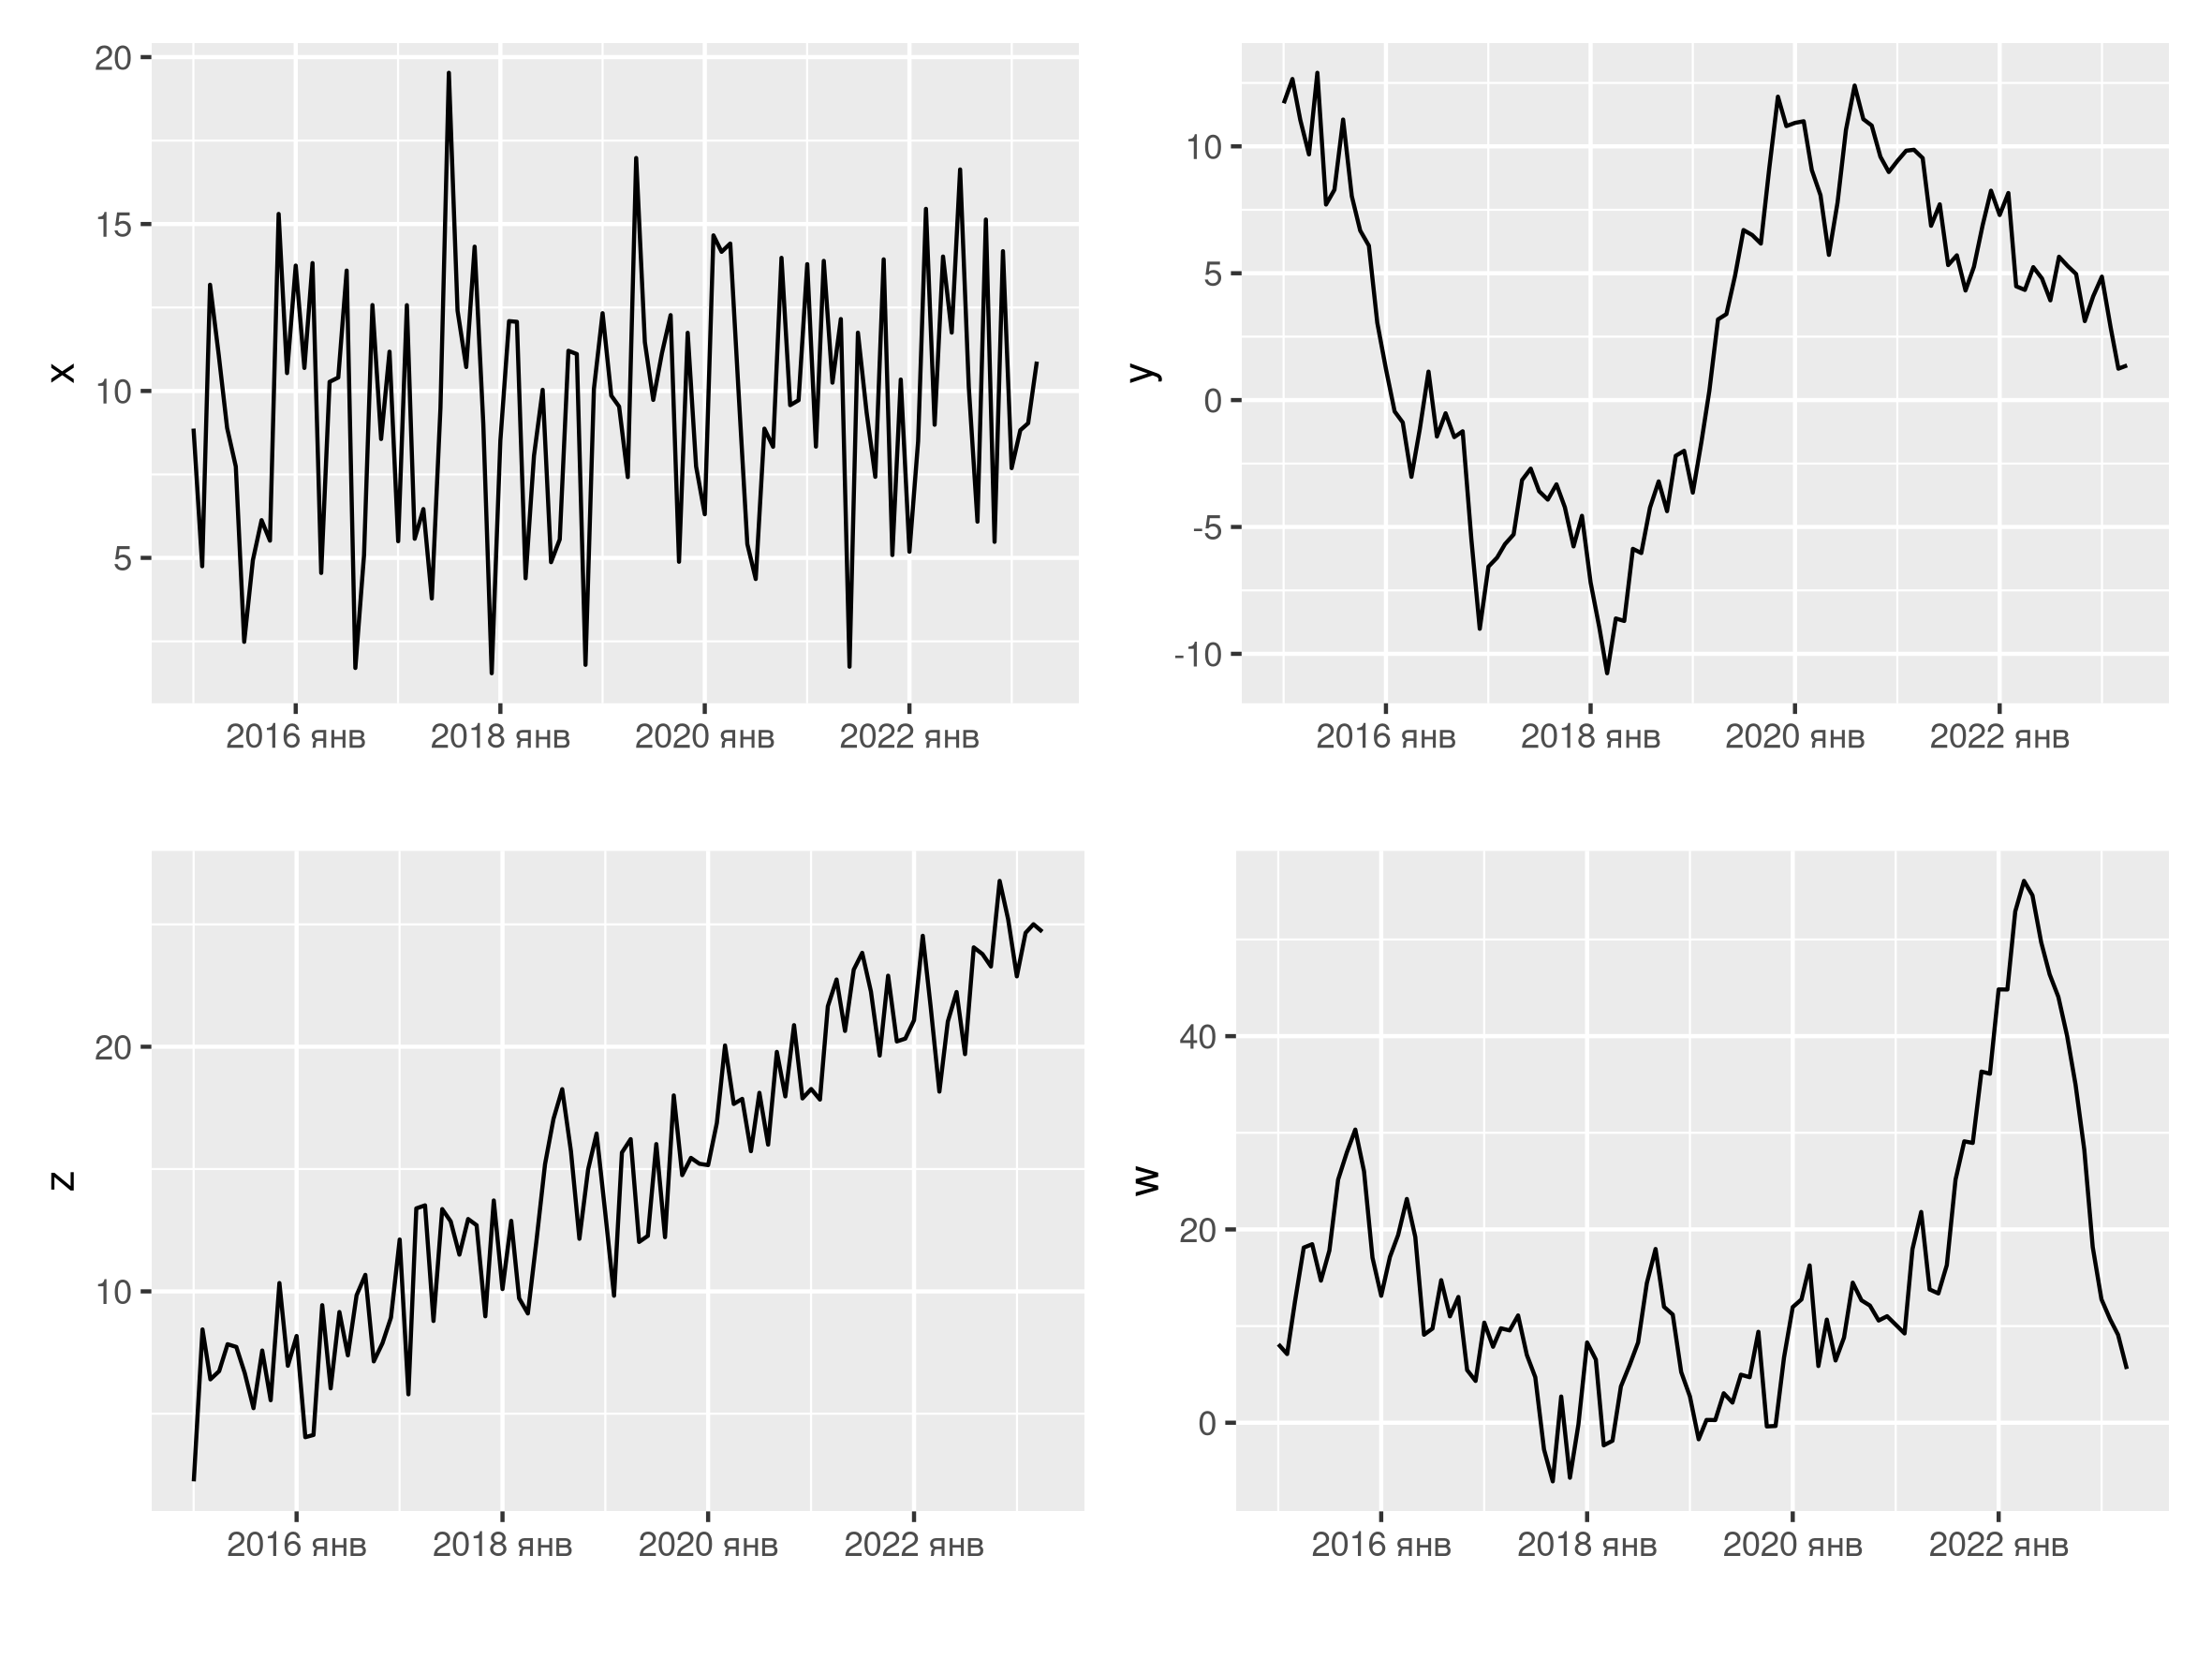
\includegraphics[width=\textwidth]{pictures/om_ts_06-027.png}
\end{frame}



\begin{frame}{Буковка I: итоги}

  \begin{itemize}[<+->]
    \item $ARMA$ подходит только для \alert{стационарных} рядов. 
    \item Иногда стационарен $\Delta y_t$ или $\Delta^2 y_t$. 
    \item Выбираем между $ARMA$ и $ARIMA$.
  \end{itemize}
\end{frame}

